\section{Exercise 17}

The nodes $A$, $B$, and $C$ of a distributed transactional system are aware of the following remote and local waiting conditions:
\begin{itemize}
    \item Node $A: E_B \rightarrow t_3, E_C \rightarrow t_2, t_1 \rightarrow E_C, t_3 \rightarrow t_5, t_5 \rightarrow t_1$
    \item Node $B: E_C \rightarrow t_2, t_3 \rightarrow E_A, t_2 \rightarrow t_3$
    \item Node $C: t_2 \rightarrow E_A, t_2 \rightarrow E_B, t_1 \rightarrow t_4, t_4 \rightarrow t_2$
\end{itemize}
Execute the Obermarck's algorithm twice, with different conventions:
\begin{enumerate}
    \item Sending messages of the form $E_X \rightarrow t_i \rightarrow t_j \rightarrow E_Y$ forward (toward node $Y$) and only if and only if $i > j$. 
    \item With the opposite conventions, so if and only if $i < j$
\end{enumerate}
Discuss the outcome, and explain it, taking into account the properties of the algorithm and the initial conditions.

\subsection*{Solution}
The graph is the following: 
\begin{figure}[H]
    \centering
    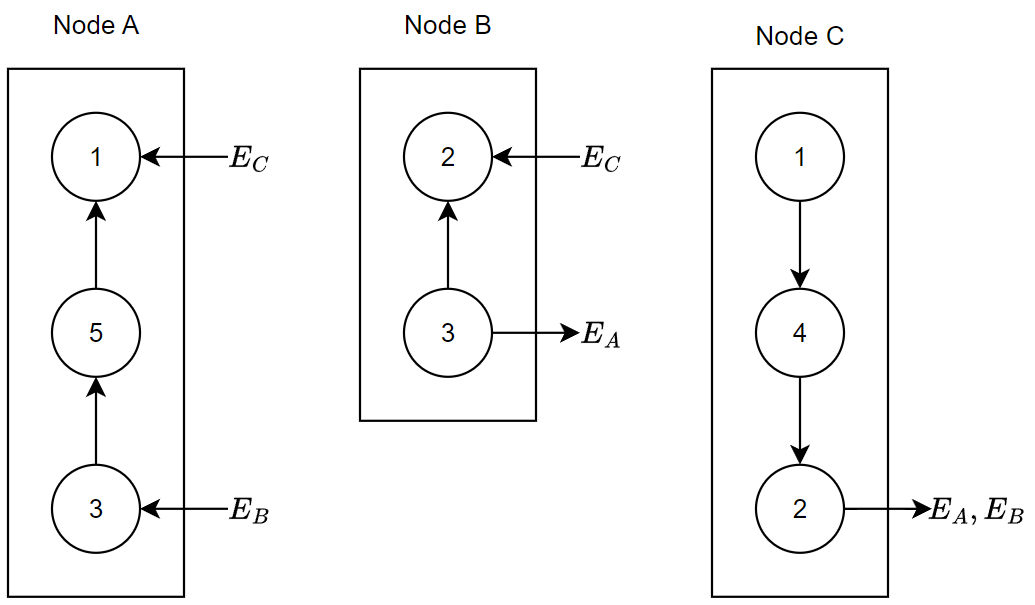
\includegraphics[width=0.75\linewidth]{images/Ob4.png}
\end{figure}
\begin{enumerate}
    \item At the first iteration we have only one arc to add, that is: $E_B \rightarrow t_3 \rightarrow t_1 \rightarrow E_C$. 
        After adding this arc and reapplying the algorithm we find the following arcs: 
        \begin{itemize}
            \item $E_B \rightarrow t_3 \rightarrow t_2 \rightarrow E_B$.
            \item $E_B \rightarrow t_3 \rightarrow t_2 \rightarrow E_A$.
        \end{itemize}
        By adding those nodes we found a deadlock. 
    \item We have to add only one node: $E_C \rightarrow t_2 \rightarrow t_3 \rightarrow E_A$.
    \item By adding this ar we have no more messages and also no cycles. 
        Therefore, there are no deadlocks. 
\end{enumerate}
The algorithm is independent of the conventions but the initial conventions, but the initial conditions must be consistent and complete. 
On a faulty dataset even the best algorithm returns untrustworthy results. 
In this case we have a link missing between node $A$ and $C$.